\begin{frame}\frametitle{Background}\framesubtitle{Softmax}
\begin{Large}
It's unsuitable to compute the softmax
\end{Large}
   \begin{equation}
  p(c|w) =  \frac{exp( {v^{'}_c}^\intercal v_w )}{\sum_{i=1}^T exp({v^{'}_i}^\intercal v_{w})}
   \end{equation}
   \begin{itemize}
   \item $v_w$ and $v^{'}_c$ are the "input" and "output" representation of $w$
\item For each pair we have to go over the whole training corpus. (Billions of word in practice) 
   \end{itemize}
\end{frame}


\begin{frame}
\frametitle{Network Architecture} 
\begin{columns}
    \column{0.6\textwidth}
\begin{itemize}
\item Dimension of input and output vectors = 100
\item Context window  = 5
\end{itemize}
    \column{0.6\textwidth}
    \begin{itemize}
    \item Negative Samples = 10 
\item Coded in Pytorch 1.0
\end{itemize}
  \end{columns}
  \bigskip
\begin{columns}
    \column{0.4\textwidth}
    		First 10 pairs of training:
        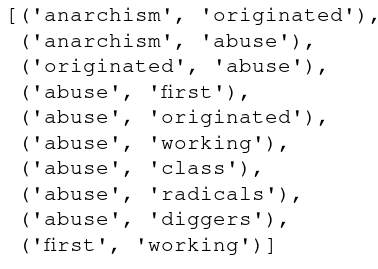
\includegraphics[scale=0.35]{images/pairs_example}    \column{0.6\textwidth}
        Negative Samples:\\
        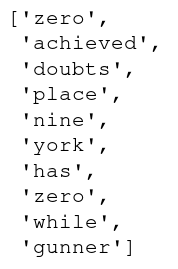
\includegraphics[scale=0.35]{images/neg_samples_example}
  \end{columns}
\end{frame}